\documentclass{beamer}
\usepackage[english]{babel}
\usepackage[utf8]{inputenc}

\usetheme{Boadilla}

\title{SAGA Async Advert Adaptor}

\author[H.C. Wilhelm]{Hans Christian Wilhelm}
\institute[hcwilhelm@mac.com]{}

\begin{document}
  
  \begin{frame}
    \titlepage
  \end{frame}
  
  \begin{frame}
    \frametitle{Table of contents}
  	\tableofcontents
  \end{frame}
  
  \section{Sync vs. Async Advert Adaptor}
    \begin{frame}{Sync Advert Adaptor}
      \begin{figure}
        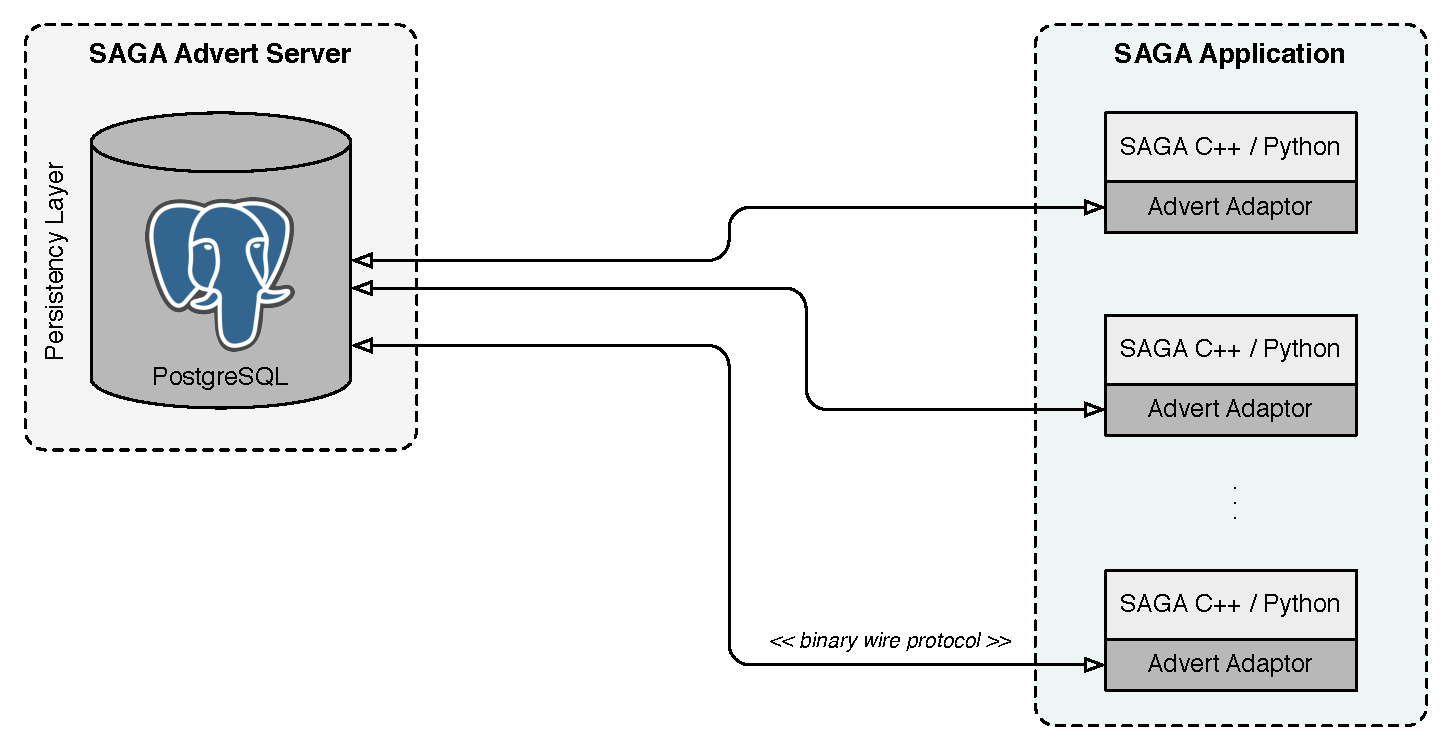
\includegraphics[width=10cm]{old_technology_overview}
        \caption{Default Advert and Fast Advert Adpator communication layout.}  
      \end{figure}
    \end{frame}
    
    \begin{frame}{Sync Advert Adaptor}
      \begin{block}{Communication layout}
        \begin{itemize}
          \item Each Adaptor instance has a single connection to the database.
          \item Directories / Entries are opened with recursive queries.
          \item This leads to multiple Request/Response roundtrips.
          \item Each Attribute needs one query.
          \item This leads to one Request/Response roundtrip per attribute.
          \item Polling is needed to see if something has changed.
        \end{itemize}
      \end{block}
      
      \begin{alertblock}{Fast Advert Adaptor}
             \begin{itemize}
               \item Reduced query count.
               \item Still needs polling !
             \end{itemize} 
      \end{alertblock}
    \end{frame}
    
    \begin{frame}{Async Advert Adaptor}
      \begin{figure}
        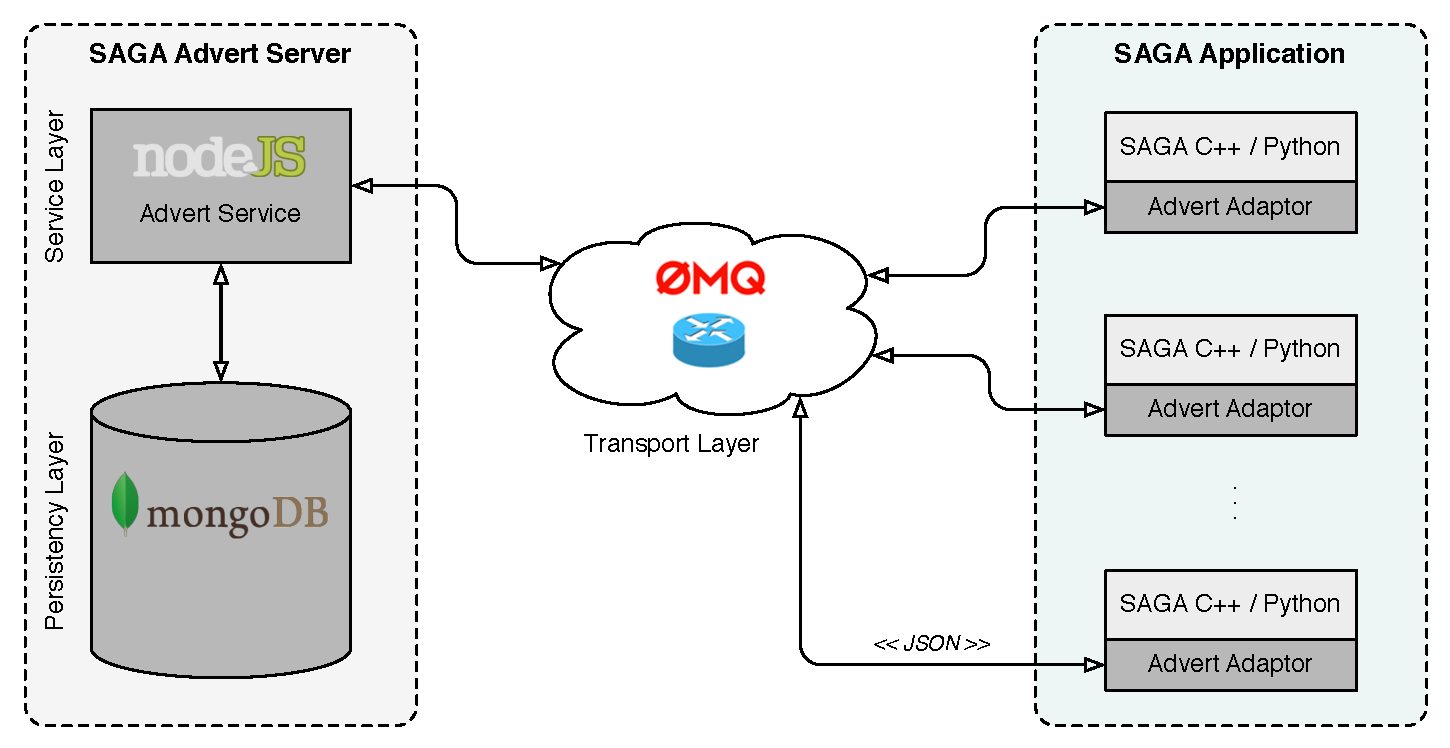
\includegraphics[width=10cm]{new_technology_overview}
        \caption{Async Advert Adpator communication layout.}  
      \end{figure}
    \end{frame}
    
    \begin{frame}{Async Advert Adaptor}
      \begin{block}{Communication layout}
        \begin{itemize}
          \item Two ZMQ connections per Adaptor instance.
          \item One Request/Response connection to send commands.
          \item One Publish/Subscribe connection to receive notifications.
          \item No recursive database layout.
          \item Directories / Entries are transported as a union.
        \end{itemize}
      \end{block}
      
      \begin{alertblock}{Roundtrips}
             \begin{itemize}
               \item Only one roundtrip to open an Diretory / Entry.
               \item No extra roundtrip to query an attribute.
               \item No polling to the server.
             \end{itemize} 
      \end{alertblock}
    \end{frame}
  
  \section{Architecture and technology}
    \begin{frame}{Architecture}
      \begin{figure}
        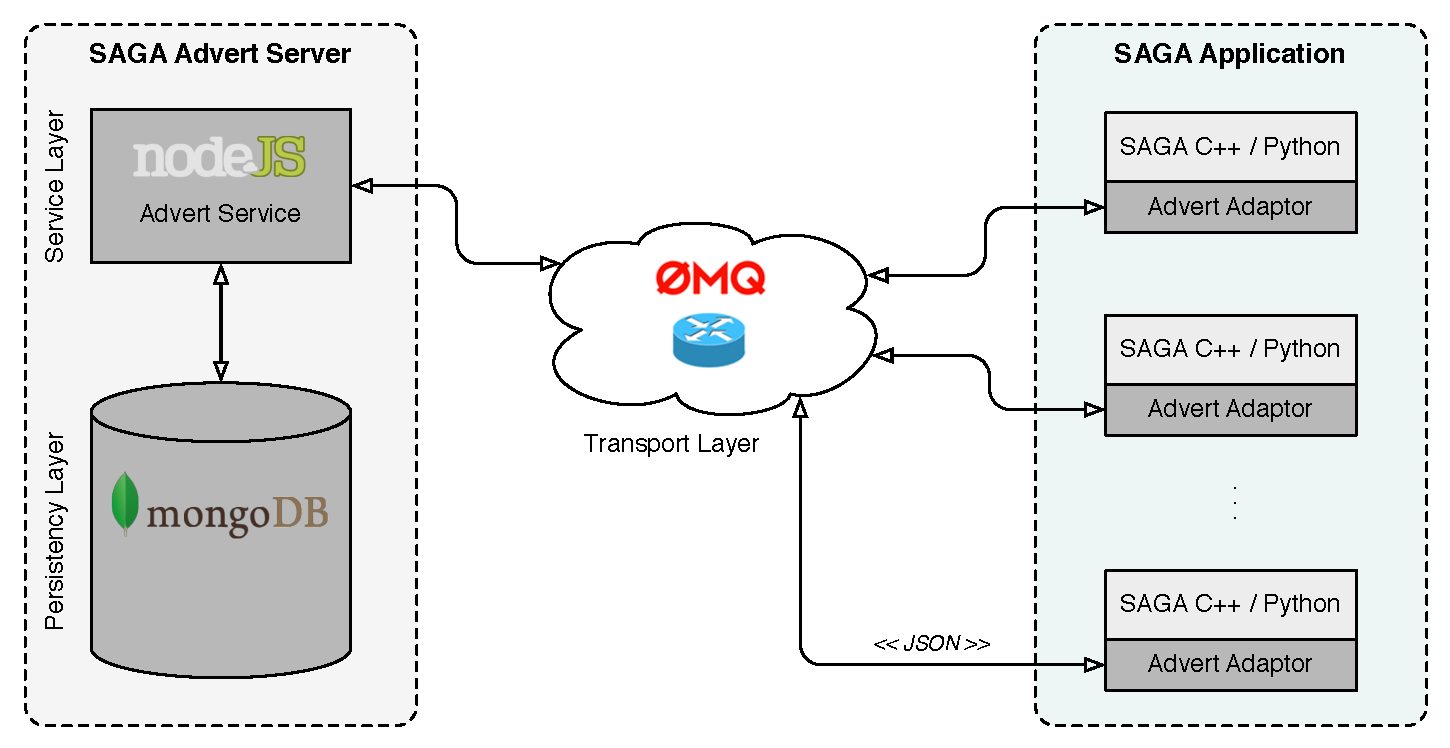
\includegraphics[width=10cm]{new_technology_overview}
        \caption{Async Advert Adpator Architecture}  
      \end{figure}
    \end{frame}
    
    \begin{frame}{Technology}
      \begin{block}{NodeJS}
        \begin{itemize}
          \item The Advert Server is implemented in the non-blocking JavaScript framework NodeJS.
          \item Manages incoming connections.
          \item Publishes messages to the Advert Adaptor client.
          \item Communicates with the Database.
        \end{itemize}
      \end{block}
      
      \begin{block}{MongoDB}
        \begin{itemize}
          \item MongoDB is used as the Database persitency layer.
          \item Document based, each directory/entry modeled as document.
        \end{itemize}
      \end{block}
    \end{frame}
    
    \begin{frame}{Technology}
      \begin{block}{ZeroMQ}
        \begin{itemize}
          \item ZeroMQ sockets connect the Advert Adaptor to the server.
          \item REQUEST/RESPONSE socket used so send commands to the server.
          \item PUBLISH/SUBSCRIBE socket used to notify the Advert Adaptor clients.
        \end{itemize}
      \end{block}
      
      \begin{block}{JSON}
        \begin{itemize}
          \item JSON is used as a lightweight data interchange format.
          \item The Advert Addaptor sends JSON coded commands e.g. Open, Close, Create to the Server.
          \item The server responds with a JSON coded diretory / entry. 
          \item The server publishes JSON coded document ID's to the Advert Adaptor Clients. 
        \end{itemize}
      \end{block}
    \end{frame}
    
    \begin{frame}{Technology}
      \begin{block}{Links}
        \begin{itemize}
          \item http://nodejs.org/
          \item http://www.mongodb.org/
          \item http://www.zeromq.org/
          \item http://www.json.org/
          \item https://github.com/JustinTulloss/zeromq.node
          \item https://github.com/LearnBoost/mongoose
          
        \end{itemize}
      \end{block}
    \end{frame}
    
  \section{Installation}
    \begin{frame}{Howto install the Async Advert Adaptor}
       \begin{alertblock}{SAGA Core}
         First make sure you have a fully working SAGA Core installation on your system ! 
         Installation details can be found on http://www.saga-project.org/documentation/installation
       \end{alertblock}
    \end{frame}
    
    \begin{frame}{Howto install the Async Advert Adaptor}
      \begin{block}{Get ZeroMQ}
        Befor the installation of the Async Advert Adaptor we need to install ZeroMQ (Release 2.1). 
        Download the POSIX tarball from http://www.zeromq.org/intro:get-the-software and install it.
      \end{block}
      
      \begin{exampleblock}{Install ZeroMQ}
         tar xvzf zeromq-2.1.10.tar.gz \newline
         cd zeromq-2.1.10 \newline
         ./configure --prefix=/choose/your/install/path/zeromq-2.1.10 \newline
         make \newline
         make install
      \end{exampleblock}
    \end{frame}
    
    \begin{frame}{Howto install the Async Advert Adaptor}
      \begin{block}{Get AsyncAdvertAdaptor}
        After the installation of ZeroMQ it is time to get the Async Advert Adpator
        from the SVN repository. 
      \end{block}
      
      \begin{exampleblock}{Install Async Advert Adaptor}
        svn co https://svn.cct.lsu.edu/repos/saga-adaptors/async\_advert\_adaptor \newline
        cd async\_advert\_adaptor \newline
        ./configure --with\_zmq=/install/path/zeromq-2.1.10 \newline
        make \newline
        make install
      \end{exampleblock}
    \end{frame}
    
  \section{Testing environment}
    \begin{frame}{Testing environment}
      \begin{block}{Testing Server}
        \begin{itemize}
          \item Async Advert testing server gw68.quarry.iu.teragrid.org
          \item sqlasyncadvert://gw68.quarry.iu.teragrid.org/
          \item Ports are hardcoded at the moment ! (5557/5558)
          \end{itemize}
      \end{block}
      
      \begin{block}{Getting started}
        \begin{itemize}
          \item Go to your SAGA Core install path /bin
          \item Play around with the saga-advert-... commands.
          \item Try the Async Advert Adaptor in your own projects.
          \end{itemize}
      \end{block}
    
      \begin{exampleblock}{Example}
        ./saga-advert-dump-directory sqlasyncadvert://gw68.quarry.iu.teragrid.org/
      \end{exampleblock}
    \end{frame}
    
    \begin{frame}{Optional Benchmark Tool}
      \begin{block}{Python Benchmark Tool}
        \begin{itemize}
          \item Install the SAGA Python bindings.
          \item Checkout the benckmark tool from https://svn.cct.lsu.edu/repos/saga-adaptors/async\_advert\_adaptor/benchmark/
          \item Have a look at the README file and start testing.
          \end{itemize}
      \end{block}
      
      \begin{exampleblock}{Example}
        \begin{itemize}
          \item svn co https://svn.cct.lsu.edu/repos/saga-adaptors/async\_advert\_adaptor/benchmark/
          \item cd benchmark
          \item python advert-benchmark.py sqlasyncadvert://gw68.quarry.iu.teragrid.org/your/benchmark/dir -p -c 10 -a 10 -i5
          \end{itemize}
      \end{exampleblock}
    
    \end{frame}
    
  \section{Effective usage}
    \begin{frame}{Effective usage}
      \begin{alertblock}{Directories / Entries are transported as unions}
        Keep in mind that directories / entries are transported as unions over the wire. That means 
        all attributes and vector attributes are transmitted with every directory / entry.
      \end{alertblock}
      
      \begin{block}{Usage hints}
        \begin{itemize}
          \item Try to keep attribute count per directoy / entry as low as possible.
          \item Don't use a single entry to coordinate all workers. 
          \item Assign every worker to it's own entry. 
          \item Try to keep entry count per directory as low as possible.
          \item Use different directories to model dependancies.
          \end{itemize}
       \end{block}
    \end{frame}
    
\end{document}